\documentclass[10pt,a4paper]{article}
\usepackage[margin=18mm]{geometry}
\usepackage{amsmath,amssymb,booktabs,array,graphicx,xcolor,fancyhdr,hyperref}
\hypersetup{colorlinks=true,urlcolor=blue,linkcolor=blue,pdftitle={BOUNDARY-11: Spherical edge extension},pdfauthor={Codex; prepared for owner and GPT review}}
\definecolor{ink}{HTML}{173247}
\pagestyle{fancy}\fancyhf{}\lhead{\small BOUNDARY-11}\rhead{\small Exact geometry / review draft}\cfoot{\thepage}
\setlength{\headheight}{13pt}\setlength{\parindent}{0pt}\setlength{\parskip}{5pt}
\newcommand{\R}{\mathbb R}\newcommand{\ez}{\mathbf e_z}\newcommand{\Rot}{\operatorname{Rot}_z}
\newcommand{\head}[1]{\vspace{4pt}{\large\bfseries\color{ink}#1}\par}
\newcommand{\smallhead}[1]{\textbf{#1}\quad}
\begin{document}
{\LARGE\bfseries\color{ink}Three-dimensional spherical edge extension}\par
{\small BOUNDARY-11 \;|\; 16 October 2026 \;|\; Mathematical construction; no physical interpretation adopted}

\textbf{Result.} The accepted shell has an exact edge-tangent sphere of radius $w/\sqrt3$.
Its 21 supporting lines give 42 distinct exits on a concentric sphere at every finite
$R\geq\rho$, except at exactly three radii, where they give 18. The complete point set
has exactly $D_{3h}$ symmetry at every such finite radius. Certain sections are regular
triangles, hexagons, octagons or 16-gons; the construction supplies no global tenfold symmetry.

\head{1. Fixed source geometry and the two natural spheres}
Use Paper C v1.0.1, \S4, with its original vertex numbering and panel maps, and
BOUNDARY-10's centred folded-shell construction. No source coordinates are fitted.
The panel width across opposite sides is $w>0$; the three panel planes meet at acute
angle $60^\circ$. The original centre and basic lengths are
\[
 o=(0,\sqrt3w/6,0),\qquad s=(\sqrt2-1)w,\qquad h=s/2,
 \qquad p=\frac{w}{2\sqrt3}.
\]
Here $p$ is the distance from $o$ to each panel plane. A regular panel's circumradius
is $\sqrt{w^2/4+h^2}$; hence every one of the 18 welded vertices satisfies
\[
 \boxed{\rho^2=p^2+w^2/4+h^2=w^2\left(\frac{13}{12}-\frac{\sqrt2}{2}\right)}.
\]
The supplied inventory preserves all 18 original and centred coordinates and the three
face cycles. Deduplicating their edges gives 21: 3 vertical weld seams, 6 horizontal
edges and 12 chamfer edges. Let $v_i,v_j$ now denote \emph{centred} endpoints of any edge.
Put $m=(v_i+v_j)/2$, $D=(v_j-v_i)/2$ and $u=D/h$. Equal endpoint norms and equal edge
lengths give, independently of orientation,
\[
 m\cdot D=\frac{\|v_j\|^2-\|v_i\|^2}{4}=0,\qquad
 \|D\|^2=h^2,\qquad \boxed{\|m\|^2=\rho^2-h^2=w^2/3}.
\]
Thus $\|m+\lambda u\|^2=w^2/3+\lambda^2$: every supporting line is tangent at its
midpoint to the concentric sphere $a=w/\sqrt3$. This is an \emph{edge-tangent midsphere},
not a face-tangent insphere: $p=a/2$, so the sphere cuts through panel interiors.
The three zero-thickness panels do not enclose a solid volume.

\head{2. Exact extension, with correspondence retained}
For every $R\geq\rho$ define $t=\sqrt{R^2-a^2}\geq h$ and $\tau=t/h\geq1$. The two exits
of each original line are exactly
\[
 \boxed{q_e^\pm(R)=m_e\pm t u_e=m_e\pm\tau D_e.}
\]
They remain on the original straight supporting line. Add $o$ to return to Paper C's
frame. Edge IDs E01--E21 use sorted original endpoint numbers; the plus sign follows
the direction from the lower numbered endpoint to the higher. All 42 labels survive
even when several exits coincide.

For a compact explicit coordinate list, let $n_k=\Rot(2\pi k/3)(0,-1,0)$,
$b_k=\Rot(2\pi k/3)(1,0,0)$, $k=0,1,2$. All independent signs below are $\pm1$:
\[
\begin{array}{ll}
\text{Seams (6):}&(a\cos\theta_j,a\sin\theta_j,0)\pm t\ez,
 \quad\theta_j=\pi/2+2\pi j/3,\ j=0,1,2;\\[3pt]
\text{Horizontal (12):}&p n_k+\epsilon t b_k+\nu(w/2)\ez;\\[3pt]
\text{Chamfer (24):}&p n_k+\displaystyle\sigma\frac{w/2+\epsilon t}{\sqrt2}b_k
 +\displaystyle\nu\frac{w/2-\epsilon t}{\sqrt2}\ez.
\end{array}
\]
These are coordinates in $\R^3$, not a planar sketch or radial projection.

\newpage
\head{3. All finite coincidences and exact angular separations}
\begin{center}
\begin{tabular}{@{}lllll@{}}\toprule
$t/w$ & $\tau$ & $R^2/w^2$ & $R/w$ (approx.) & Unique points\\\midrule
$(\sqrt2-1)/2$ & $1$ & $13/12-\sqrt2/2$ & $0.613373094$ & 18\\
$1/2$ & $1+\sqrt2$ & $7/12$ & $0.763762616$ & 18\\
$(1+\sqrt2)/2$ & $3+2\sqrt2$ & $13/12+\sqrt2/2$ & $1.338073284$ & 18\\\bottomrule
\end{tabular}
\end{center}
At each event there are 12 double points and 6 triple points, giving $12(2)+6(3)=42$
labelled incidences. At the first event the points are exactly the original vertices.
At every other allowed finite radius there are 42 distinct points.

\smallhead{Exhaustiveness proof.}
Within each panel the eight support lines are tangent to its incircle of radius $w/2$,
with successive normals $\pi/4$ apart. Nonparallel pairs meet at local distances
\[
 L=\frac{w}{2}\sec\frac{\pi}{8},\quad
 \frac{w}{2}\sec\frac{\pi}{4},\quad
 \frac{w}{2}\sec\frac{3\pi}{8}
\]
from the panel centre. Since $R^2=p^2+L^2$, these give precisely the table.
Two different panel planes meet only along their shared vertical seam line. All
nonparallel edge-line crossings on that seam have heights
$z=\pm h,\ \pm w/2,\ \pm(1+\sqrt2)w/2$, yielding the same three radii.
Distinct parallel lines do not meet; skew lines do not meet. This covers every pair.
At each event each panel contributes eight distinct points. The six seam points
belong to two panels, so their union has $3(8)-6=18$ points. Each non-seam point
joins two support lines, and each seam point joins three. The exact symbolic scan of
all 861 branch pairs, checked against all 210 line pairs, agrees with this argument.

\smallhead{Angles.}
For labels $(e,\epsilon)$ and $(f,\delta)$ the central spherical angle is uniquely
specified in $[0,\pi]$ by
\[
 \cos\gamma=\frac{m_e\cdot m_f+
 t(\epsilon u_e\cdot m_f+\delta u_f\cdot m_e)
 +\epsilon\delta t^2u_e\cdot u_f}{R^2};\qquad \text{arc length}=R\gamma.
\]
This gives every pair exactly. The machine-readable catalogue records all 861 pairs
in 60 symbolic function classes, as $(A+B\tau+C\tau^2)/(1/3+h_1^2\tau^2)$ for $w=1$,
$h_1=(\sqrt2-1)/2$. Function values can merge at special radii; 60 is not claimed as
a fixed count of numerical angle values. In particular,
\[
 \gamma(q_e^+,q_e^-)=2\arctan(t/a),\qquad
 \cos\gamma_{\rm seam\ neighbours}=1-\frac{w^2}{2R^2}.
\]
The seam triangles have azimuthal step $120^\circ$, but this is not their spherical
central angle. All three of their chord sides equal $w$, for every $R$.

\head{4. Symmetry is preserved, and does not increase at finite radius}
The rotations by $120^\circ$, vertical reflections and reflection $z\mapsto-z$
permute the original edges and therefore their exits for every $R$.
For the generic 42-point set its second moment about $o$ is
\[
 \sum_q qq^{\mathsf T}=
 \operatorname{diag}(12t^2+4w^2,\ 12t^2+4w^2,\ 18t^2+6w^2).
\]
The distinct vertical eigenvalue forces every symmetry to preserve the vertical
axis. For each exceptional 18-point set, summing \emph{unique} points instead gives
$M_{zz}-M_{xx}=3w^2/2>0$, so the same conclusion holds. The level $z=t$ contains just
the three seam points (additional labels only coincide there at the listed events).
Its equilateral triangle restricts the horizontal action to $D_3$; the sign of $z$
allows at most another factor two. All 12 actions already exist: the full symmetry
is exactly $D_{3h}$. Generic orbit sizes are $6,12,12,12$; event orbit sizes are
$6,12$; $6,6,6$; and $6,12$, respectively.

\newpage
\head{5. Rings and naturally arising polygons}
Set $f_\pm=(w/2\pm t)/\sqrt2$. Latitude is $\arcsin(z/R)$.
\begin{center}
\begin{tabular}{@{}lll@{}}\toprule
Edge family & Signed heights & Points per signed level, generically\\\midrule
Seams & $\pm t$ & 3 (regular triangle)\\
Horizontal & $\pm w/2$ & 6\\
Chamfer & $\pm f_+$ & 6\\
Chamfer & $\pm f_-$ & 6\\\bottomrule
\end{tabular}
\end{center}
Generically these are eight levels; $f_-$ may be negative. Shared levels occur at
the three tabulated events, with zero latitude at the middle event. A six-point
$D_3$ ring need not be a regular hexagon.

\smallhead{Exact horizontal hexagons.}
A ring of the form $p n_k\pm u b_k$ is a regular hexagon when
$|u|=p/\sqrt3=w/6$ (its six sorted azimuth gaps then equal $60^\circ$).
For the $z=\pm f_+$ chamfer rings, $u=f_-$, so this occurs at
\[
 \frac{t}{w}=\frac12\pm\frac{\sqrt2}{6},\qquad
 \frac{R^2}{w^2}=\frac{23}{36}\pm\frac{\sqrt2}{6},\qquad
 \frac{R}{w}\simeq0.634969785,\ 0.935195781.
\]
Each hexagon has circumradius and chord side $w/3$. These are equation-defined
section events, not preferred enclosing radii; the full set still has 42 points
and only $D_{3h}$ symmetry.

\smallhead{Complete sections in each original panel plane.}
The intersection circle has radius $L=\sqrt{R^2-p^2}$. Its exit angles, measured
about the panel centre, are $\theta_0+k\pi/4\pm\beta$, where
\[
 \beta=\arccos\frac{w}{2L},\qquad \pi/8\leq\beta<\pi/2.
\]
At $\beta=\pi/8,\pi/4,3\pi/8$ the 16 labels become eight regularly spaced points:
the three coincidence events. Connecting them along the \emph{original support lines}
gives, respectively, a convex octagon, two squares, and the octagram $\{8/3\}$.
Otherwise each panel circle has 16 distinct points. The two shifted octagonal sets
interlace regularly exactly when $2\beta$ is an odd multiple of $\pi/8$ modulo $\pi/4$.
In the permitted range this yields regular 16-gons at
\[
 \beta\in\{3\pi/16,5\pi/16,7\pi/16\},\qquad
 \frac{R^2}{w^2}=\frac1{12}+\frac1{4\cos^2\beta},
\]
with $R/w\simeq0.667044981,0.945140485,2.579121735$. Polygon sides between consecutive
points are a derived adjacency, not additional edges of the shell. These panel
circles are small circles on the sphere, not great circles.

\smallhead{Limit, not an extra finite event.}
As $R\to\infty$, $q_e^\pm/R\to\pm u_e$. The limiting direction set has 20 distinct
points: two poles, six equatorial directions and six at each latitude $\pm45^\circ$.
Its symmetry increases to $D_{6h}$ (a unique vertical second-moment axis, a regular
equatorial hexagon, and both reflection types). Parallel directions merge only
in this limit. Twenty points do not imply tenfold symmetry.

\head{6. Radial comparison and limits of interpretation}
Radially projecting the original vertices gives $r_i(R)=(R/\rho)v_i$: 18 points with
unchanged angular separations and $D_{3h}$ symmetry. At $R=\rho$ this agrees with the
edge exits. For $R>\rho$ a projected endpoint cannot remain on its own edge line:
its perpendicular component is $(R/\rho)m$, whereas every point of that line has
component $m\ne0$. Projecting an entire edge gives a great-circle arc, not its
straight spatial extension. The viewer shows these vertex projections as orange crosses.

\textbf{Conclusion for discussion.} The exact edge-tangent sphere and the whole
parameter family are justified by the accepted geometry. No radius selection,
physical outer boundary or tenfold structure follows from them. The tenfold
conclusion here concerns the whole set, its native-axis latitude rings and complete
panel-circle sections; arbitrary specially selected subsets were not exhaustively
classified. All polygon observations above are geometric consequences, not new
physics, dynamics or closure rules.

\newpage
\head{7. Static views of the genuine three-dimensional construction}
\begin{center}
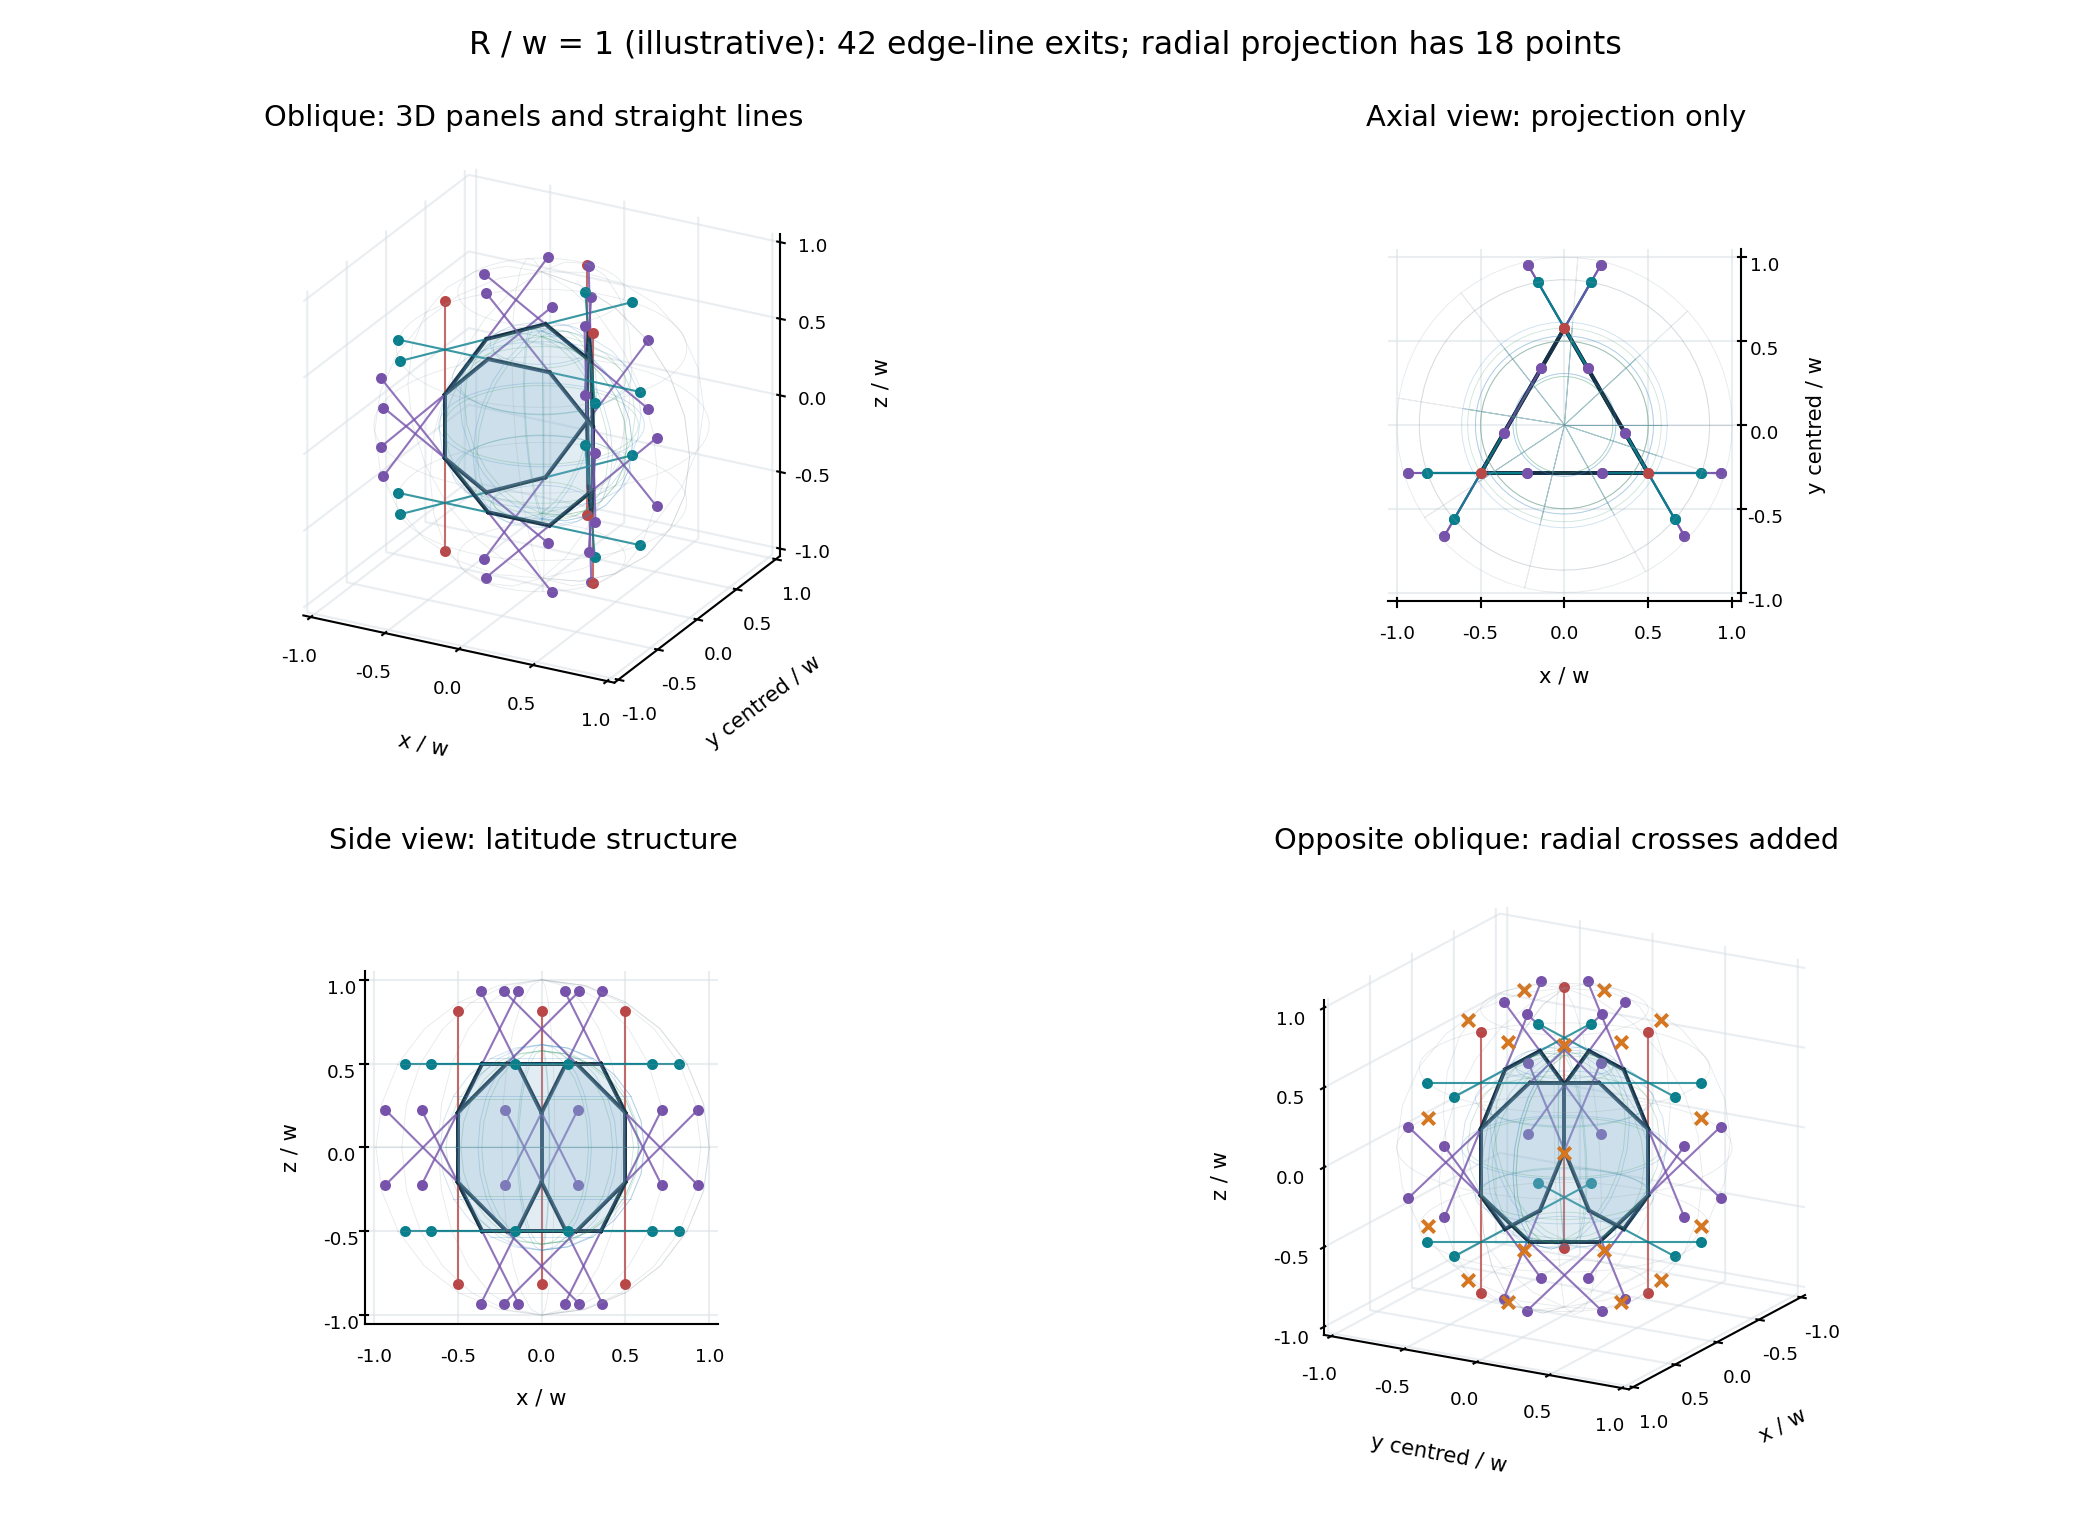
\includegraphics[width=\linewidth]{figures/01_static_views.png}
\end{center}
\textbf{Figure 1.} Four views at the illustrative value $R/w=1$. Original edges are
dark; extended seam, horizontal and chamfer lines are red, teal and violet.
The inner edge-tangent sphere is green, the vertex sphere blue and the selected
enclosing sphere grey. Orange crosses in the last view are the secondary radial
projection. All panels and all 21 edges are retained. Apparent crossings in an
axial or side projection need not be coincidences in space.

\head{Interactive viewer}
Open \texttt{BOUNDARY11\_VIEWER.html} in a WebGL-capable browser. It is a local,
self-contained file with its plotting library embedded; no server or network
connection is needed. Drag to rotate and scroll to zoom. Change $R/w$, select an
edge to highlight its two exits, or use the three exact-event buttons. Individual
layers, midpoint markers and radial crosses can be toggled. Hovering a dot shows
all incident edge labels; export retains all 42 labelled rows even at coincidences.

The slider covers $\rho/w$ to 3; the number field admits larger radii. The displayed
point count uses tolerance $10^{-9}\max(1,R/w)$ and can merge unresolved points near
an exact event or at very large radii. The symbolic classification on page 2 defines
the mathematical count. The initial radius 1 is only a viewing choice. No time
evolution or simulation is performed.

\newpage
\head{8. Event views, latitude trajectories and review evidence}
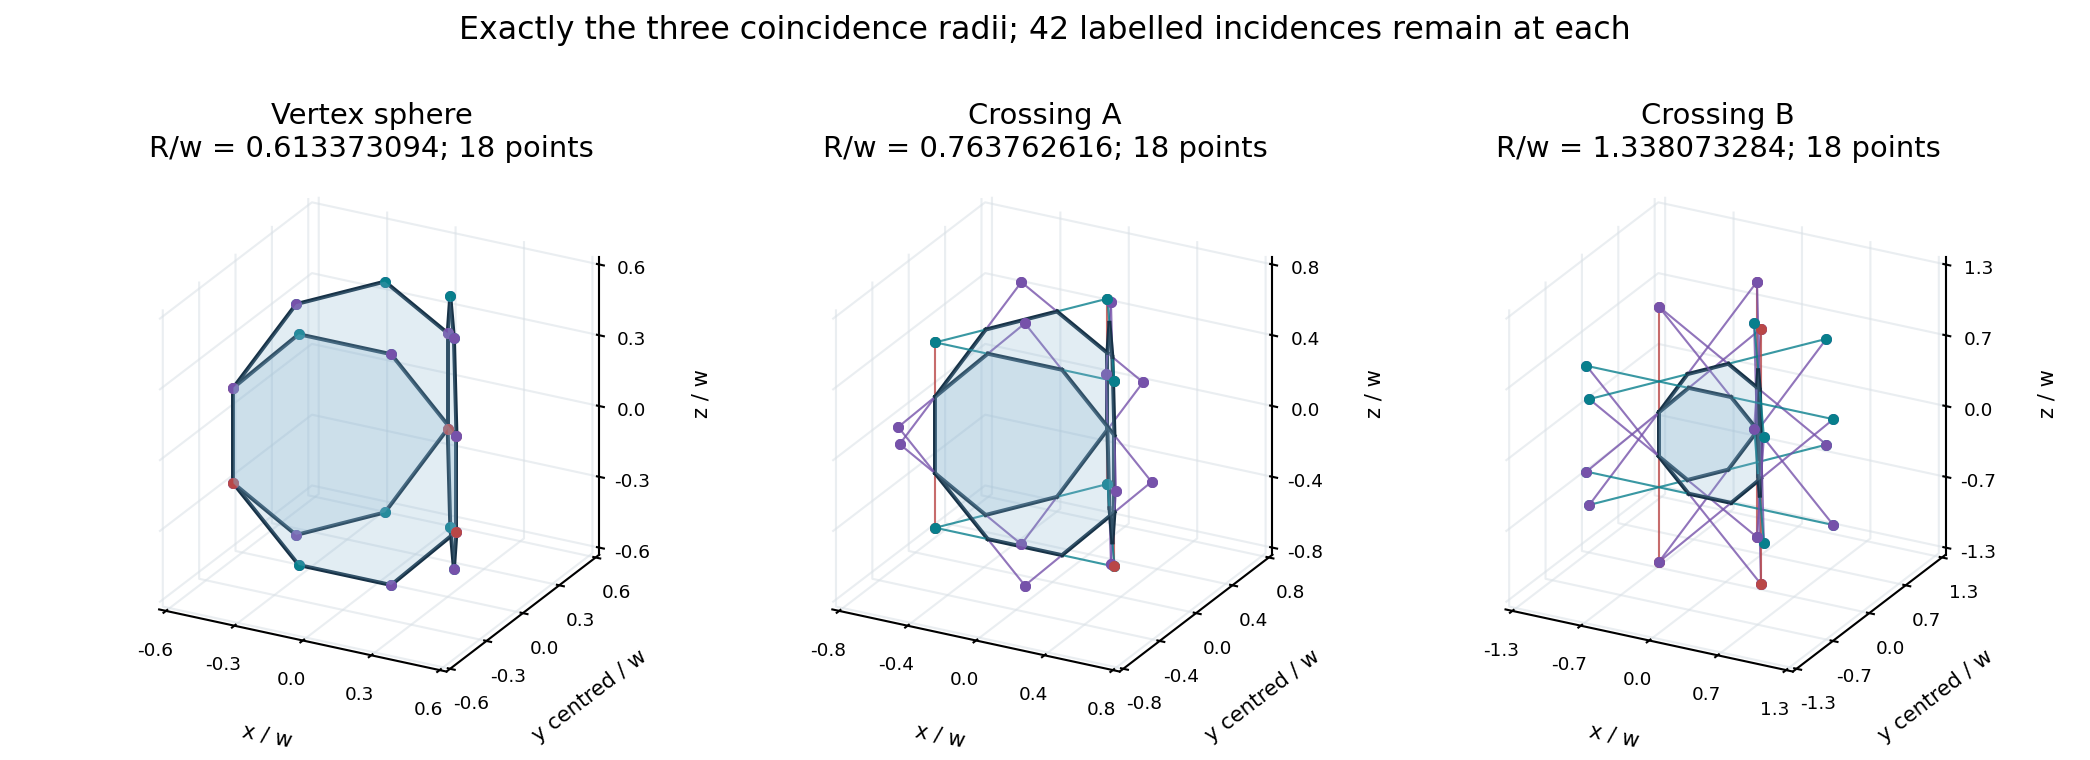
\includegraphics[width=\linewidth]{figures/02_coincidence_spheres.png}

\textbf{Figure 2.} The three and only three finite coincidence spheres, in the
same orientation. Each has 18 unique points but 42 edge incidences. Each view is
scaled to its own enclosing sphere; apparent panel sizes therefore differ.

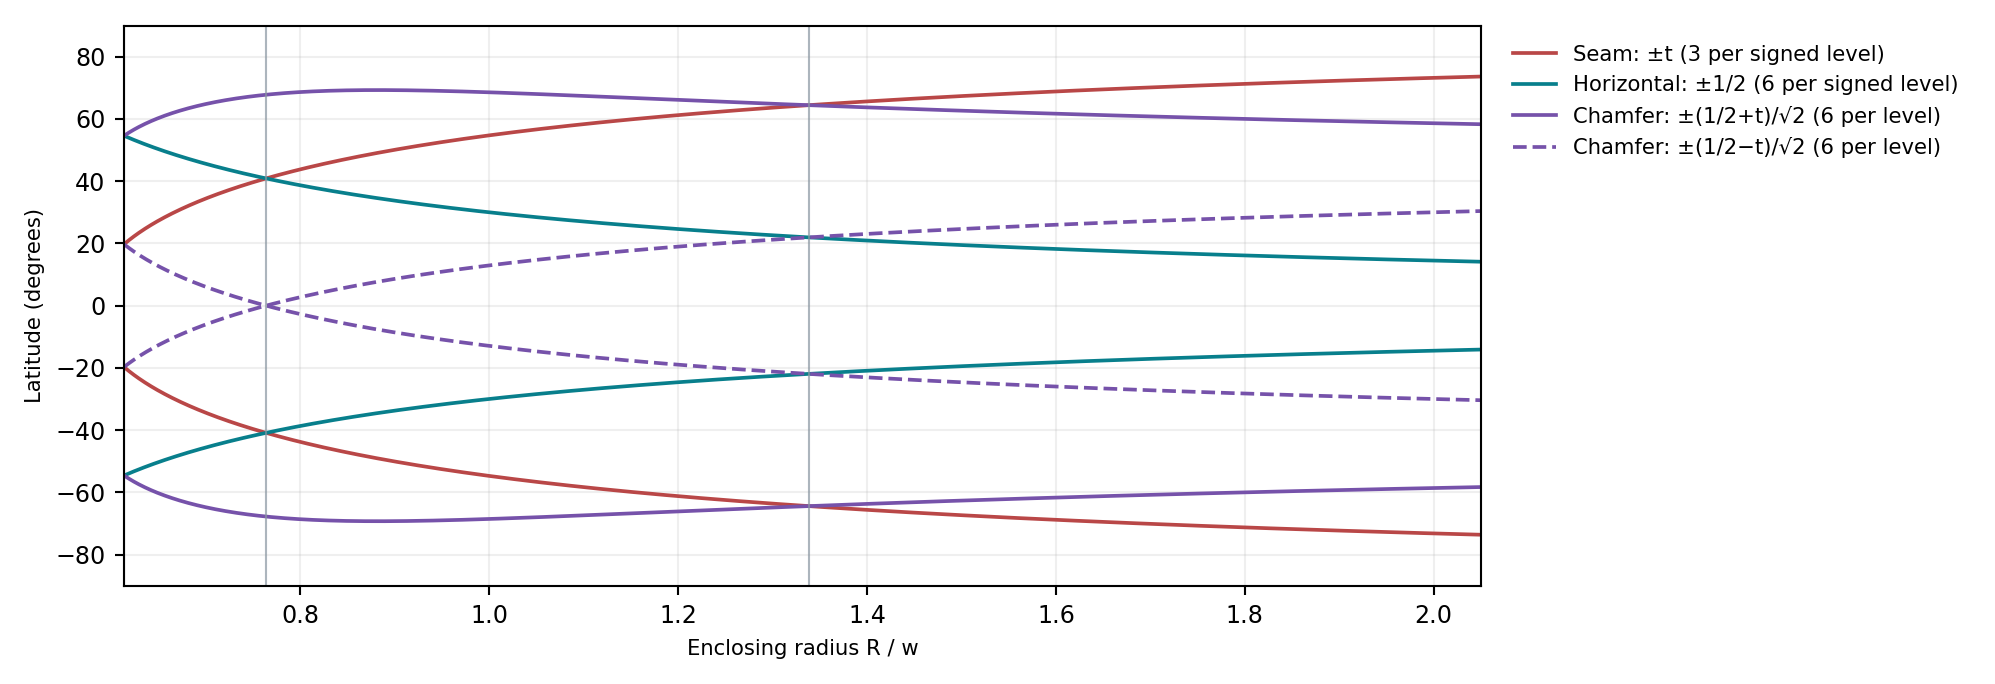
\includegraphics[width=\linewidth]{figures/03_latitude_families.png}

\textbf{Figure 3.} Latitude families as the enclosing radius varies, with $w=1$
in the legend. Vertical guides mark the three exact coincidence radii. The curves
are evaluations of the explicit coordinate formulas, not a dynamical trajectory.
Per-level counts are generic; event coincidences reduce the number of unique dots.

\smallhead{Sources reused.}
Paper C, \emph{Exact Tri-Octagon Geometry}, v1.0.1, \S4 (accepted coordinates, panel
maps and face cycles), at \texttt{papers/PAPER\_C/publication/v1.0.1/} in the local
\texttt{trioctagon-physics} repository; and \texttt{research/BOUNDARY10\_20261016/BOUNDARY10\_REPORT.tex}
and its PDF (centred shell and enclosing-sphere context). The source identity ledger
records their full paths and SHA-256 values. No new source census or earlier
polygon investigation was repeated. The new identities are proved above.

\smallhead{Reproducible evidence.}
\texttt{analyze.py} reconstructs the 18 numbered vertices independently from the
three accepted local panel maps, verifies all edge midpoint identities, scans all
861 branch pairs and all 210 line pairs, and checks the symbolic $D_{3h}$ action.
Its evidence file records 161 passing predicates. \texttt{patterns.py} checks
the event orbit sizes and polygon relations. \texttt{build\_visuals.py} generates
the three PNG/SVG plates and the standalone viewer from the same exact inventory.

\texttt{data/geometry\_inventory.json} supplies every edge's endpoints, midpoint,
unit direction and event correspondence; \texttt{data/angular\_separations.json}
supplies every angular pair. The numerical figure checks have maximum spherical
residual $2.23\times10^{-16}w$ across six test radii. The actual viewer mathematics
is also compared to those independent Python evaluations. These finite numerical
checks support the implementation; the proofs establish the parameter-wide results.

All work is isolated under \texttt{research/BOUNDARY11\_20261016/}. Python was run
in the requested \texttt{torment} Conda environment using Command Prompt. No project
scientific modules were imported or modified. This deliverable is for owner and
GPT review; no kernel, SRG, accepted paper, Git or publication action is included.
\end{document}
